%\documentclass{sig-alternate}
\documentclass[11pt]{article}
\usepackage{apacite}
\usepackage{graphicx}
\usepackage{subfig}
\usepackage{float}
\usepackage{array}
\usepackage{titlesec}



%\newcommand{\IGNORE}[1]{}
%\title{\vspace{-2cm} Adversarial Training \vspace{.5em} \rule{\textwidth}{}\vspace{.2em} \hrule}

\title {\vspace{-3cm}
		\rule{\textwidth}{2.0pt}
		\textbf{Adversarial Training}
		\rule{\textwidth}{0.5pt}
}


\author{
  \textbf{Hammad Hassan} \\
  University of Richmond \\
  hammad.hassan@richmond.edu
}
\date{July 11 2018}

\begin{document}

\maketitle
\begin{abstract}
  A brief (one paragraph) description of the work you did.
\end{abstract}


\section{Introduction}
Computer vision is currently one of the growing fields in computer science. Convolutional neural networks are trained on data and used to detect and classify objects and images. Currently, convolutional neural networks are used in a variety of applications around us such as self-driving cars, autonomous drones and facial detection software. However, the security of such networks may be compromised. Images can be perturbed to add specific noise, imperceptible to the human eye which can be used to fool these networks. These perturbed images are termed as adversarial images. This paper investigates whether injecting such adversarial examples in the training data leads to a more robust network and analyses the feasibility of this approach. Previous researchers have investigated the outcome on MNIST data set as well as on Imagenet images. This paper seeks to explore the outcome of adversarial training on an image classifier whose training data has been collected and labeled by the experimenters themselves. 


\section{Related Work}

Work has been done to classify bird into their respective species. In \cite{berg2013you}, Berg and Belhumeur construct an image recognition
system with the goal of explaining to birders the differences between similar species. \\ \\
Ian J Goodfellow with his colleagues at Google \cite{kurakin2016adversarial} explored the feasibility of injecting adversarial images in training data set using Imagenet images. He understood that for one-step attacks, the method was helpful and made the classifier more robust. \\ \\
In \cite{madry2017towards}, the MIT research team explores the security measures which may be taken to counter the adversaries and explain various methods which are feasible.

\section{Methods}
\label{sec:methods}

The experiment was designed to test the impact of injecting adversarial images in the training data of a convolutional neural network. Images of birds were collected and labeled. These images were then split into training, validation and test set. A neural network was trained on these images. Afterwards, the foolbox library in python was used to generate adversarial images for each of the bird category. The network was further trained on these adversarial images and the results were noted. 


\subsection{Image Collection}

Images were collected using two motion-activated wildlife cameras, a Wingscapes BirdCam 2.0 and (when the original failed) a Wingscapes Birdcam Pro. The
specifications and settings used are summarized in Table \ref{table:cameras}.
\begin{table}[H]
  \caption{Camera descriptions}
  \label{table:cameras}
  \begin{center}
    \begin{tabular}{|>{\footnotesize}l|>{\footnotesize}c|>{\footnotesize}c|}
      \hline
      & \bf{Birdcam 2.0} & \bf{Birdcam Pro} \\ \hline
      \bf{Max resolution} & 8.0 MP & 20.0 MP \\ \hline
      \bf{Res. used} & medium & medium \\ \hline
      \bf{Dimensions} & 2048 x 1536 & 2112 x 1188 \\ \hline
    \end{tabular}
  \end{center}
\end{table} 

\noindent The images were collected
in Richmond, Virginia, USA, over a period of six months from
March through August of 2014. The images
were collected at the camera's medium resolution setting. This level of
resolution is not needed for the automatic classification of images,
as the resulting number of parameters in the neural net is too large
to be computationally feasible on available computing resources.
However, the higher resolution was helpful in some cases for humans
doing the initial labeling of the training data sets.
The target was an upright suet feeder with a
tail-prop, a configuration favored by woodpeckers. An opaque shield
was mounted behind the feeder to provide a uniform background for the
images. The shield and feeder were painted with Krylon Neon Green paint.
Neon green was chosen because none of the species that typically feed
as this type of feeder have any green in their plumage, making it more
difficult to confuse background pixels with pixels belonging to the
bird in background removal algorithms. The feeder, shield and camera
were mounted on a pole equipped with a squirrel baffle. The camera was
attached to the pole by an adjustable arm, sold as an accessory by
Wingscapes.\\ \\
The cameras have various settings controlling focus,  sensitivity to motion
and how the camera responds when motion is detected. The camera does not
autofocus; rather, it has a series of selectable fixed focus distances.
The shortest focus distance puts the focus point at approximately the
back of the feeder with the arm fully extended in our setup, which means
that, especially in low light situations where depth-of-field is shallow,
the bird is not in sharp focus. Experimentation revealed that the most
sensitive setting for motion detection was set off even by vibrations
in the shield caused by wind, resulting in hundreds of images of an
empty feeder. Consequently, the camera was set at medium sensitivity,
and was programmed to capture three images for each motion detected
event, followed by a 30 second pause before sensing for motion again.
Some species, like Carolina Chickadees and Tufted Titmice, perch,
procure a beak-full of food, and are off immediately. Other species,
such as Carolina Wrens and the woodpeckers, perch and stay on the
feeder for extended periods of time. As a result, the size of useful
training and validation sets exhibited a very wide range across categories.\\ \\
Not all species present in the area where the images were collected
visit feeders, and of those that do, not all visit the style of
feeder used in this study. A total of 20 species visited
the feeding station during the data collection period. Of those,
twelve species were present in enough images to be useful for
training and validating a classifer. The set of species used in the
training data is shown in Table \ref{table:species}.
\begin{table}[H]
  \small
  \caption{Training set species}
  \label{table:species}
  \begin{center}
    \begin{tabular}{l}
      \hline
      %\bf{Training set species} \\ \hline 
      Brown Thrasher \\ 
      Carolina Chickadee \\ 
      Carolina Wren \\ 
      Downy Woodpecker  \\
      European Starling\\
      GrayCat Bird\\ 
      Northern Cardinal \\ 
      Red-bellied Woodpecker \\ 
      Tufted Titmouse \\ 
      White Breasted Numthatch\\
      White Throated Sparrow\\
      Yellow Rumped Warbler \\ \hline
    \end{tabular}
  \end{center}
\end{table}
A thirteenth category of images of an empty feeder
was also added. \\ \\
Two typical images are show in figure \ref{fig:TypicalImages}.

\begin{figure}[H]
  \centering
  \subfloat[Soft shadows]{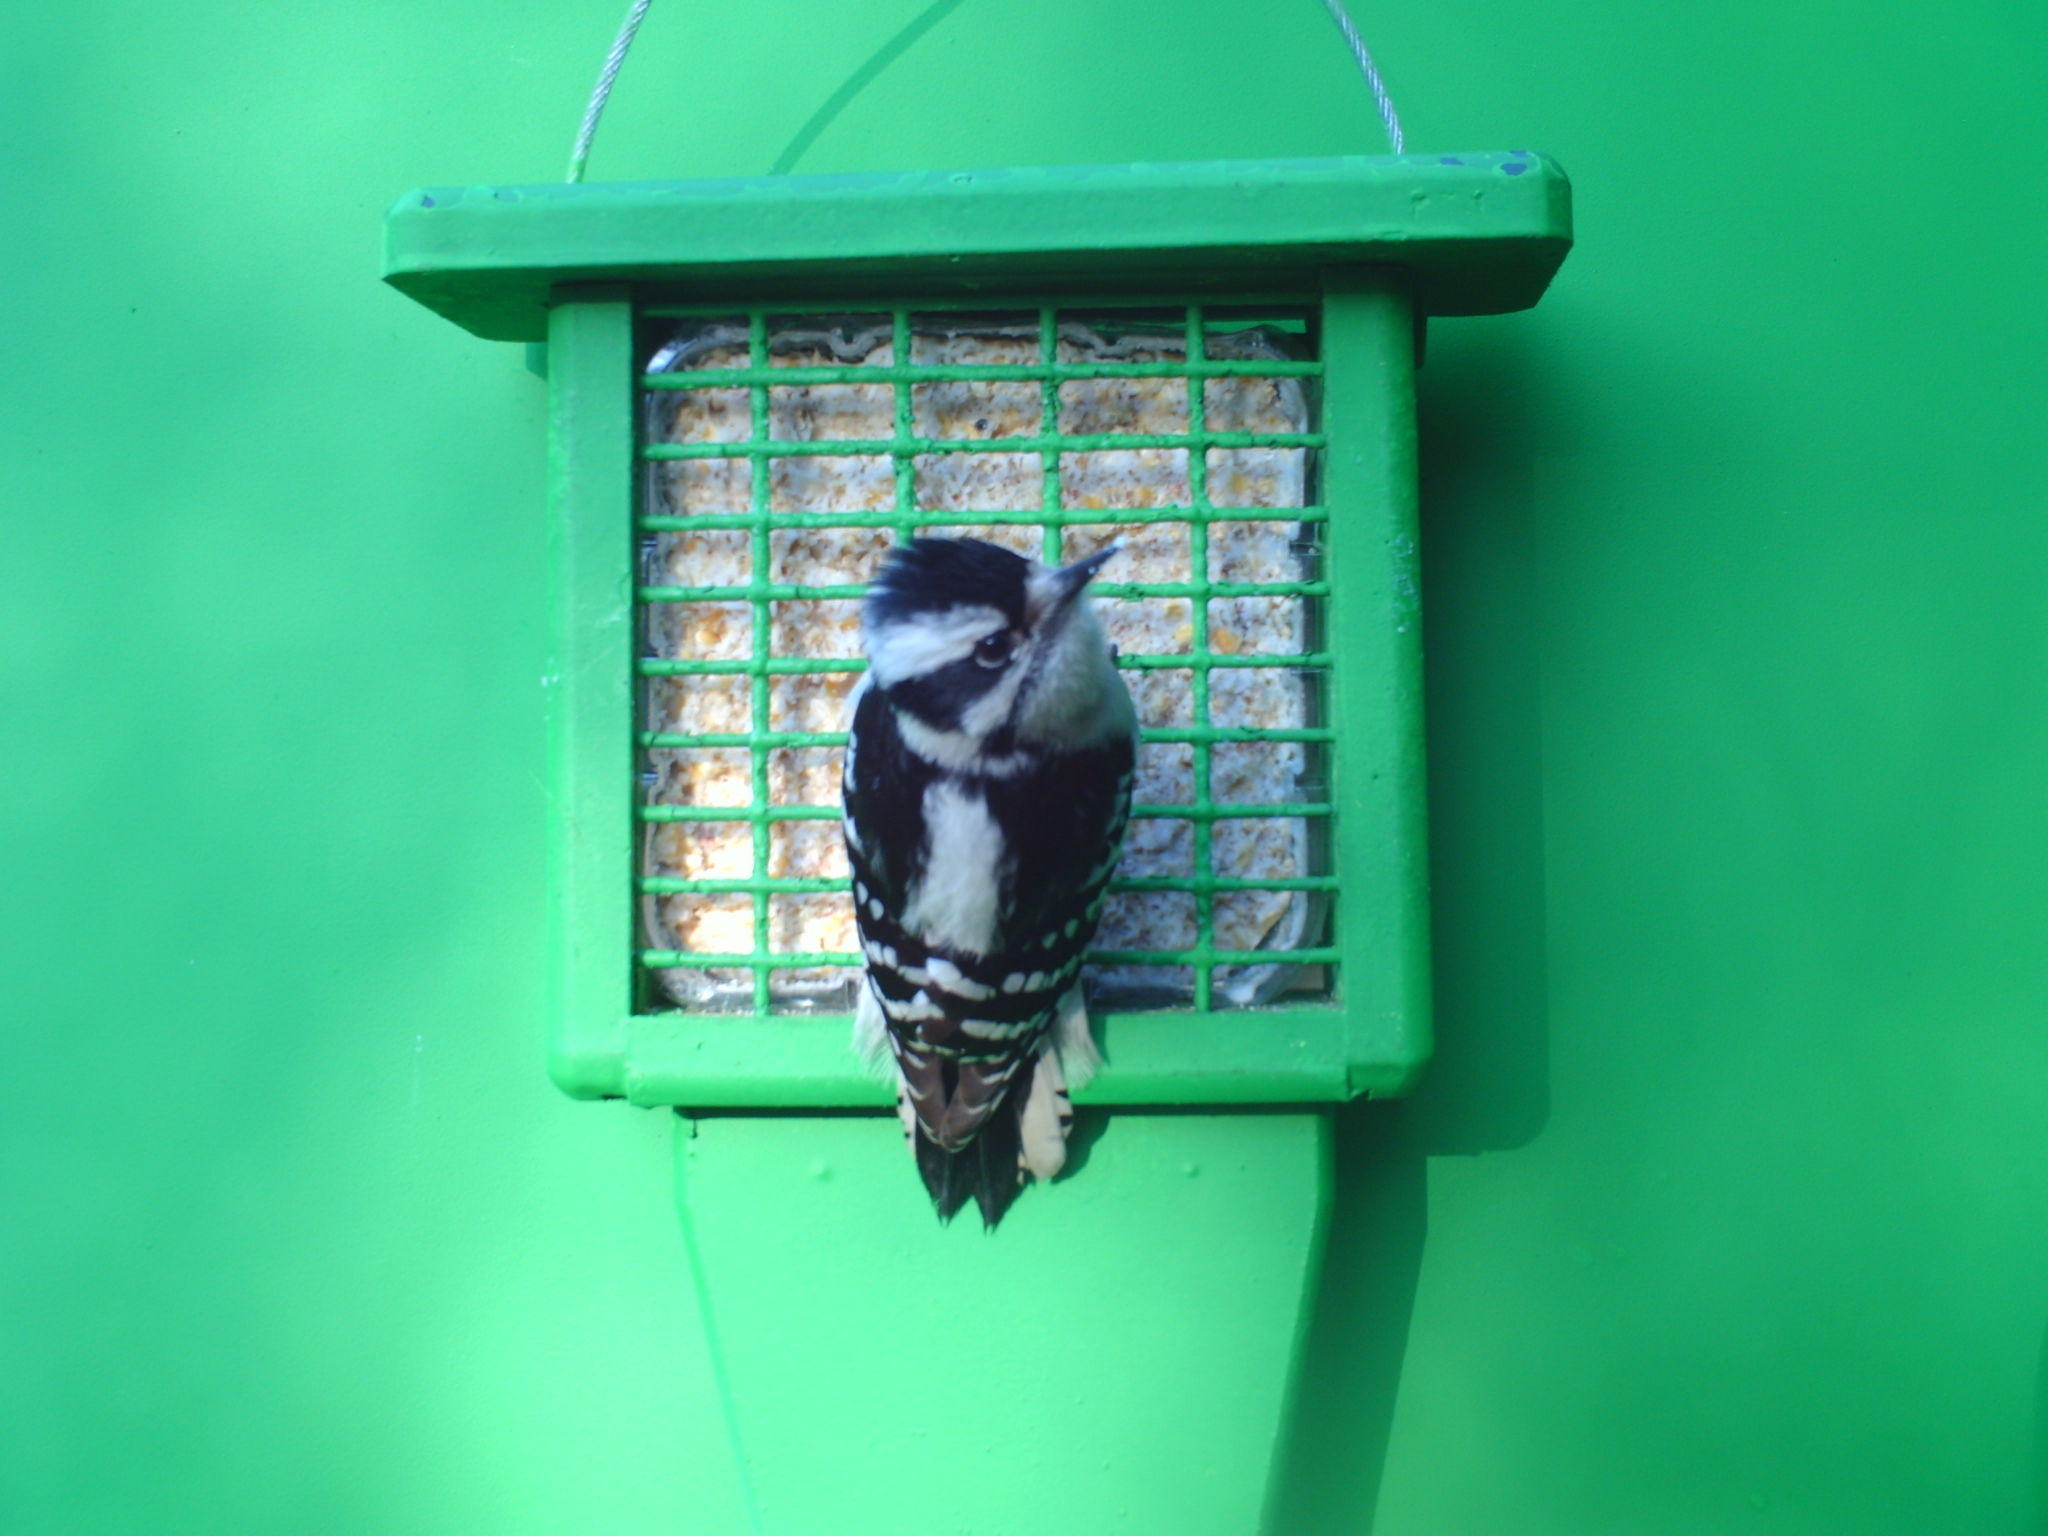
\includegraphics[width=1.5in]{images/typical.jpg}}
  \hspace*{1em}
  \subfloat[Hard shadows]{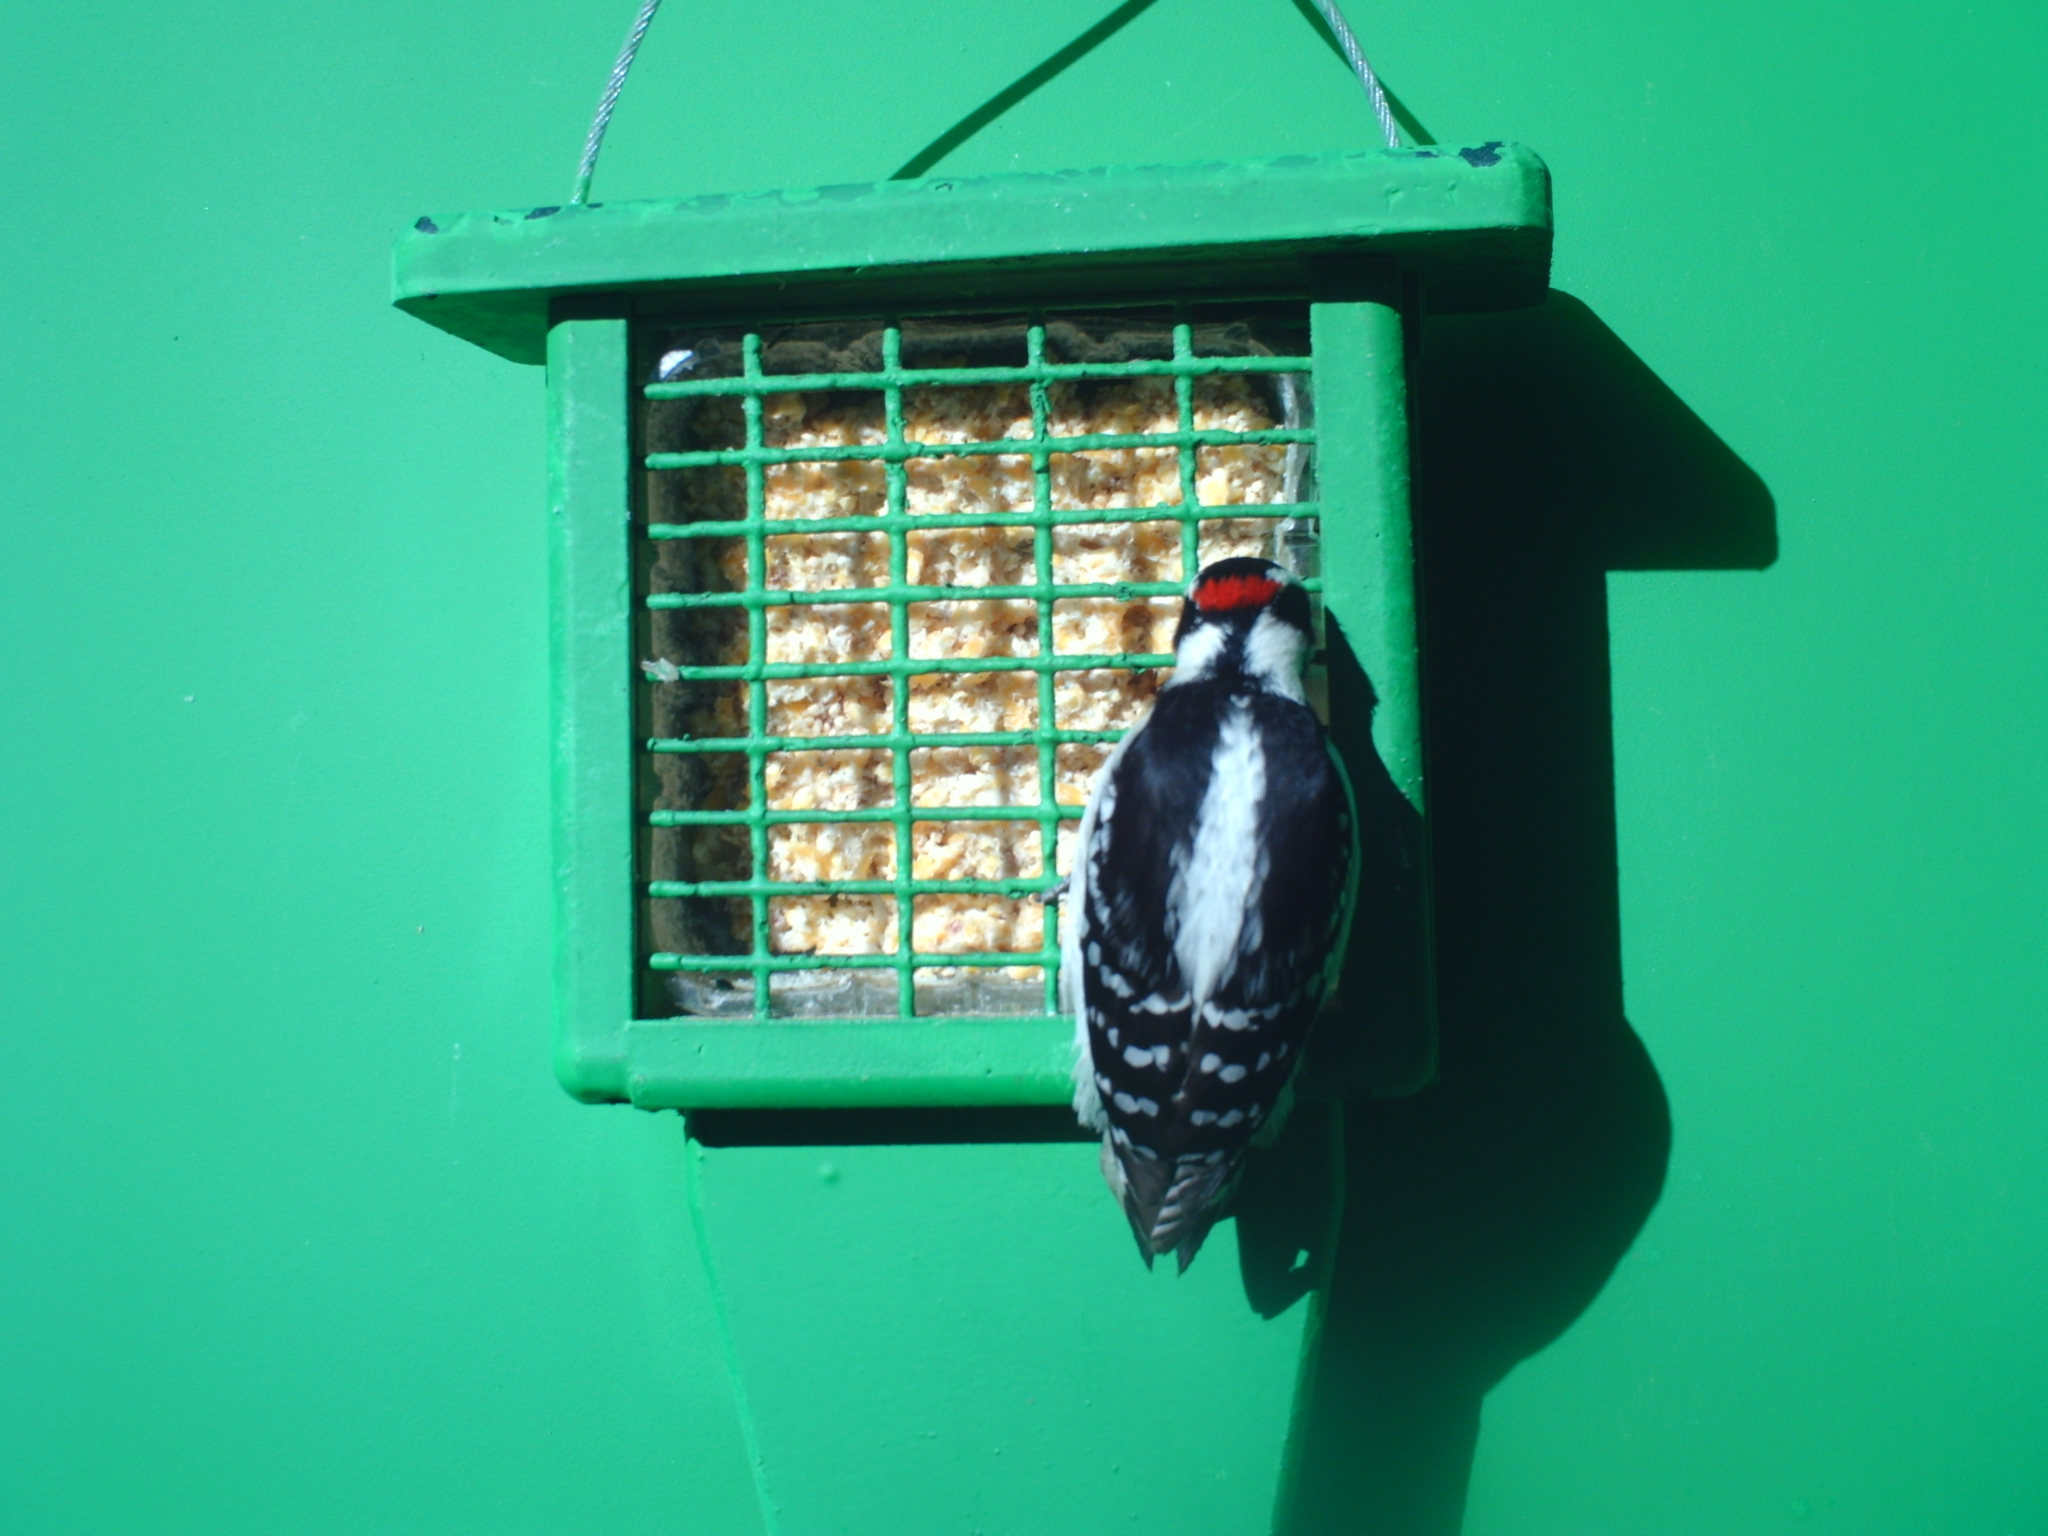
\includegraphics[width=1.5in]{images/bright.jpg}}
  \caption{Some typical images. \label{fig:TypicalImages}}
\end{figure}


The images collected were split into three subsets: 
\begin{itemize}
	\item
	Training
	\item 
	Validation
	\item 
	Test
\end{itemize}
Eighty percent of the images in each category were randomly selected for training set, fifteen percent for validation and the remaining five percent were used for test.  
\subsection{Convolutional neural network architecture and Training}

The Keras library with tensorflow backend was used to build the classifier. The network architecture used was as follows:

\begin{center}
\begin{table}[H]
 \begin{tabular}{||c c c c||} 
 \hline
  & \textbf{Layer(type)} & \textbf{Filters/Pool Size/units} & \textbf{Activation Function} \\ [0.5ex] 
 \hline\hline
  & Convolutional $2D$ & $32$ & $relu$ \\ 
 \hline
  & Convvolutional $2D$ & $32$ & $relu$ \\
 \hline
  & MaxPooling$2D$ & $(2,2)$ & \\ 
 \hline
 & Dropout & $0.15$ &\\
 \hline
 & Convolutional $2D$ & $64$ & $relu$ \\ 
 \hline
  & Convvolutional $2D$ & $64$ & $relu$ \\
 \hline
  & MaxPooling$2D$ & $(2,2)$ & \\ 
 \hline
 & Dropout & $0.15$ &\\
 \hline
 & Convolutional $2D$ & $256$ & $relu$ \\ 
 \hline
  & Convvolutional $2D$ & $256$ & $relu$ \\
 \hline
  & MaxPooling$2D$ & $(2,2)$ & \\ 
 \hline
 & Dropout & $0.15$ &\\
 \hline
 & Flatten  &&\\
 \hline
 & Fully Connected Layer & $1024$ & $relu$\\
 \hline
 & Dropout & $0.15$ & \\
 \hline
 & Fully Connected Layer & $13$ & $softmax$\\
 \hline
\end{tabular}
\caption{The network architecture}
\end{table}
\end{center}

\noindent The images were presorted into their specific directory of train, validation and test and each directory had subfolders of the category for the respective images. This allowed the Keras method $flow \ from \ generator$ to be used to produce hot-encoded labels. A hot-encoded label assigns an integer value to each of the categories from $0-12$. It acts like a map where each category is mapped to an integer value. Thus the classifier would return an array of length $13$, of predictions for each image, each index representing the probability that the image belongs to that respective category. The network was trained for a total of forty epochs. The accuracy and results of the classifier are shown below:
\begin{table}[H]
\begin{center}
	
		\begin{tabular}{||c c c ||}
			\hline
			& \textbf{Training Accuracy} & $93.2$\\
			\hline
			& \textbf{Validation Accuracy} & $93.3$\\
			\hline
			&\textbf{Test Accuracy} & $94.5$\\
			\hline
			& \textbf{Test Loss} & $0.37$\\	
			\hline
	
		\end{tabular}	
		\caption{Accuracy results}
	
\end{center}
\end{table}
\subsection{Adversarial Image Generation}
The idea behind adversarial image generation is to alter the pixel data of the image very minutely to ensure that it gets misclassified. For an image classifier $M$, assume that $M(x) = y \textsubscript{true}$ where $x$ is an input image and $y\textsubscript{true}$ is the original class of the image. We need to generate an adversarial image $x'$ such that $M(x') \neq y\textsubscript{true}$ where $x'$ is the adversarial example and $x'$ and $x$ are indistinguishable for the human. To do this, a random class $y'$ is selected from the output classes such that $y'\neq y\textsubscript{true}$. Gradient descent is applied to the input pixels of $x$ in order to minimize the classification loss with respect to the newly chosen class. To ensure that the adversarial looks like the original image, distance is used.Therefore, perturbation $r$ is assigned a very small value. This basically means the value by which each pixel may be altered. So the adversarial image $x' = x + r$. Since $|r|$ is as small as possible, $|x-x'|$ is minimized and the image generated looks very similar to the original image. The $|x-x'|$ is one example of distance minimized to produce adversarial images. There are many distances which may be used to ensure that the adversarial image looks very similar to the original image. Some examples may include $L \inf$, $Mean \ Squared \ Distance $ and $ L_0$ distance. Minimizing this distance ensures that the adversarial image is indistinguishable fron the original.\\ \\
The foolbox library developed by Bethge Lab was used to generate adversarial images \cite{rauber2017foolbox}. This library comes pre-loaded with a wide variety of attack strategies. The original network was loaded. The criteria for each attack was defined using Target Class Probability. The target class was randomly selected from any of the classes except the original one and the target probability was set to 0.95. This ensured that the adversarial created would fool the network easily. The Linfinity distance was used which calculates $L\infty$ norm distance $d(x, y) \ = \ max_i|x_i-y_i|$ where $x$ and $y$ are two vectors, the original image and the adversarial image respectively. The attack method used was the Projected Gradient Descent. It calculates the gradient with respect to the input pixels in an image and applies sign operation to that image. The threshold of the gradient matrix is taken and multiplied by a small number epsilon and then added to the image. In this experiment, epsilon was set at $0.0003$ Once the adversarial meets the criteria, the image is returned. 
The images were saved as $.png$ files with their original names as well their targeted class name for example $2014-03-17 \ 17.19.08\_GrayCatBird.png$. An example of adversarial images is shown below:
 
\begin{figure}[H]
  \centering
  \subfloat[Original Image]{\includegraphics[width=1.5in]{images/Original(BrownThrasher).jpg}}
  \hspace*{1em}
  \subfloat[Adversarial Image misclassified as Tufted Titmouse]{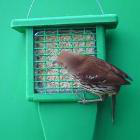
\includegraphics[width=1.5in]{images/Adversarial(TuftedTitmouse).png}}
  \caption{An adversarial example of Brown Thrasher.  \label{fig:TypicalImages}}
\end{figure}

The predictions for the above images are as follows:
\begin{figure}[H]
\centering
\includegraphics[scale=1.0]{images/Original_predictions.png}
\caption{Original image prediction}
\end{figure}
\begin{figure}[H]
\centering
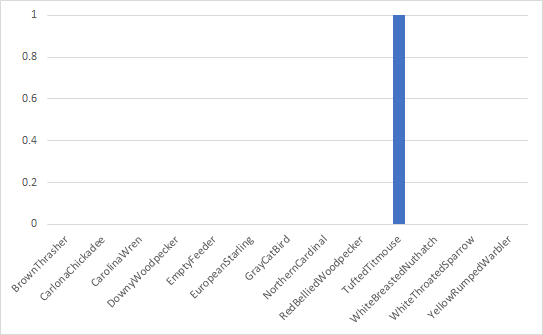
\includegraphics[scale=1.0]{images/Adversarial_predictions.png}
\caption{Adversarial image prediction}
\end{figure}

\noindent The adversarial images were also arranged into their respective directories. The adversarial images were similarly split as the original data into train, validation and test. The train and validation sets were mixed with the original ones while the test sets were kept separately. A new network was then trained on these data sets. Both the original and this new adversarial network were tested on both of the test sets.
\section{Results}
The results of the accuracy of the networks on the test sets are shown below:
\begin{table}[H]
	\begin{center}
		\begin{tabular}{||c c c||}
		\hline
		& \textbf{Original Network} & \textbf{Adversarial Network}\\
		\hline
		\textbf{Original Data} & $94.5$ & ...\\
		\hline
		\textbf{Adversarial Data} & ... &...\\
		\hline
		\end{tabular}
	\end{center}
\end{table}


\label{sec:results}

Describe how things worked.

\section{Discussion}

This section usually talks about {\em why} the results came out
as they did.

\section{Conclusions}


\section{Acknowledgments}
The author gratefully acknowledges the support of
the University of Richmond Undergraduate Research Committee,
Robert Plymale, Dr. Lewis Barnett and Hadi Abdullah.

\newpage

\bibliographystyle{apacite}
\bibliography{References}

\end{document}
